\section{Experiments}
\label{sec:exp}

\subsection{Data and protocol}
\label{sec:data}
We use the Passive Vehicular Sensors (PVS) dataset~\cite{menegazzo2021pvs}: nine trips in which three vehicle--driver pairs each drove the same three routes (10.7, 11.6 and 13.8~km).
Each vehicle carries fixed IMU modules on the dashboard and above and below the suspension, a GNSS receiver at 1~Hz, and video from which the speed bumps, the surface type (asphalt, cobblestone, dirt) and the road quality of each side (good, regular, bad) were annotated.
We use the left logger only (the two loggers have separate clocks that drift by up to 0.54~s) and its dashboard IMU, the closest proxy for a phone in a holder; the modules are not phones.
To compare vehicles at the same places, each trip's GNSS fixes are matched in time order to the first vehicle's track within a forward window (the routes are loops, so nearest-point matching would confuse start and end).
Matched fixes lie a median 1.5--3.8~m from the reference track, and 97.9--99.3\% of samples are matched.
Routes are cut into 100~m stretches, and a place enters the analysis if all three vehicles covered it at a mean speed of at least 5~m\,s$^{-1}$, RoadScribe's own floor for road values: 310 places.
The video labels agree across the three trips of a route (weighted $\kappa=0.93$), so they serve as a vehicle-independent reference.

Hypotheses, thresholds and analyses for the cross-vehicle study were fixed and committed to the project repository before the vibration data were analysed; analyses added afterwards are marked as exploratory.
Confidence intervals are from a block bootstrap over contiguous 1~km blocks of places (2{,}000 resamples), which respects spatial autocorrelation.

\subsection{Narrator benchmark}
\label{sec:bench}
\TBD[: Table with T, T+V, S-PGR (regenerated with a sufficient token budget): acceptance, claims per narrative, $P_L$, H1 by cluster bootstrap over drives, grounding against labelled bumps with random-placement control.]

\subsection{Are road claims vehicle-invariant?}
\label{sec:invariance}
Table~\ref{tab:invariance} compares RoadScribe's two kinds of per-stretch claim across the three vehicles at the same places.
Felt classes \emph{should} differ, because comfort depends on the vehicle and the speed.
Road classes are presented as properties of the road and should agree.
They do not: the road class differs between two vehicles at the same place in 76\% of pairs (by two or more classes in 14\%), all three vehicles give the same road class at only 4.5\% of places, and the weighted $\kappa$ is 0.72 [0.60, 0.76].
In a regression of the log road value on place and vehicle fixed effects and log speed, the vehicle alone accounts for 18.2\% [14.3, 27.5] of the variance.
Shuffling the vehicle labels within places 1{,}000 times gives 0.06\% on average (99th percentile 0.27\%), so this vehicle signature is not an artefact of the analysis.
The speed-decoupled road value is no more vehicle-invariant than the felt value (vehicle share 18.8\%), and only 2.1\% of the variance is a place-by-vehicle interaction: the vehicles differ mainly by a constant factor.

\begin{table}[t]
\caption{Agreement of per-stretch claims across the three vehicles at 310 places (dashboard IMU). $\kappa$: mean pairwise quadratic-weighted Cohen's kappa of the six comfort classes; vehicle share: unique variance explained by the vehicle in log value $\sim$ place + vehicle + log speed. Brackets: 95\% block-bootstrap intervals.}
\label{tab:invariance}
\centering
\small
\begin{tabular}{@{}lcccc@{}}
\toprule
Claim & $\kappa$ & all three agree & pairs differ & vehicle share \\
\midrule
Felt ($a_v$) & 0.66 [0.53, 0.72] & 9.7\% & 66\% & 18.8\% \\
Road ($\tilde a_w$, Eq.~\ref{eq:dec}, $\gamma=0.35$) & 0.72 [0.60, 0.76] & 4.5\% & 76\% & 18.2\% [14.3, 27.5] \\
Road, calibrated (Eq.~\ref{eq:cal}) & \TBD & \TBD & \TBD & \TBD \\
\bottomrule
\end{tabular}
\end{table}

\paragraph{Sensor placement (exploratory).}
The size of the vehicle signature depends on where the sensor sits.
For the module above the suspension it is small (vehicle share 2.9\%, road $\kappa=0.86$), and for the module below the suspension it is 11.8\% ($\kappa=0.60$).
The dashboard, the placement closest to a phone in a holder, is the worst of the three.

\subsection{Speed}
\label{sec:speed}
Fig.~\ref{fig:speed} plots the weighted vertical vibration of each place and vehicle against speed.
Pooled across places, vibration \emph{falls} with speed (slope $-0.64$): the slow places are the rough ones.
Within a place, net of vehicle, it rises with slope $+0.86$ (the difference is 1.50 [1.26, 1.64]).
The sign reversal comes mostly from surface type: cobblestone and dirt stretches are driven slowly, and within each surface the pooled slope is positive (asphalt $+0.16$, cobblestone $+0.54$, dirt $+1.36$; exploratory).
Even within asphalt, however, the across-place estimate is about 80\% smaller than the within-place one ($+0.16$ versus $+0.96$).
The value $\gamma=0.35$ in RoadScribe's default configuration was estimated in this across-place way, on asphalt with trip fixed effects (0.32 and 0.36 for the two dashboard bands); with it, the road value still rises with speed at a fixed place (slope 0.51).
A speed elasticity for decoupling has to be estimated from repeated passes over the same places, as in Eq.~\eqref{eq:fe}.

\begin{figure}[t]
\centering
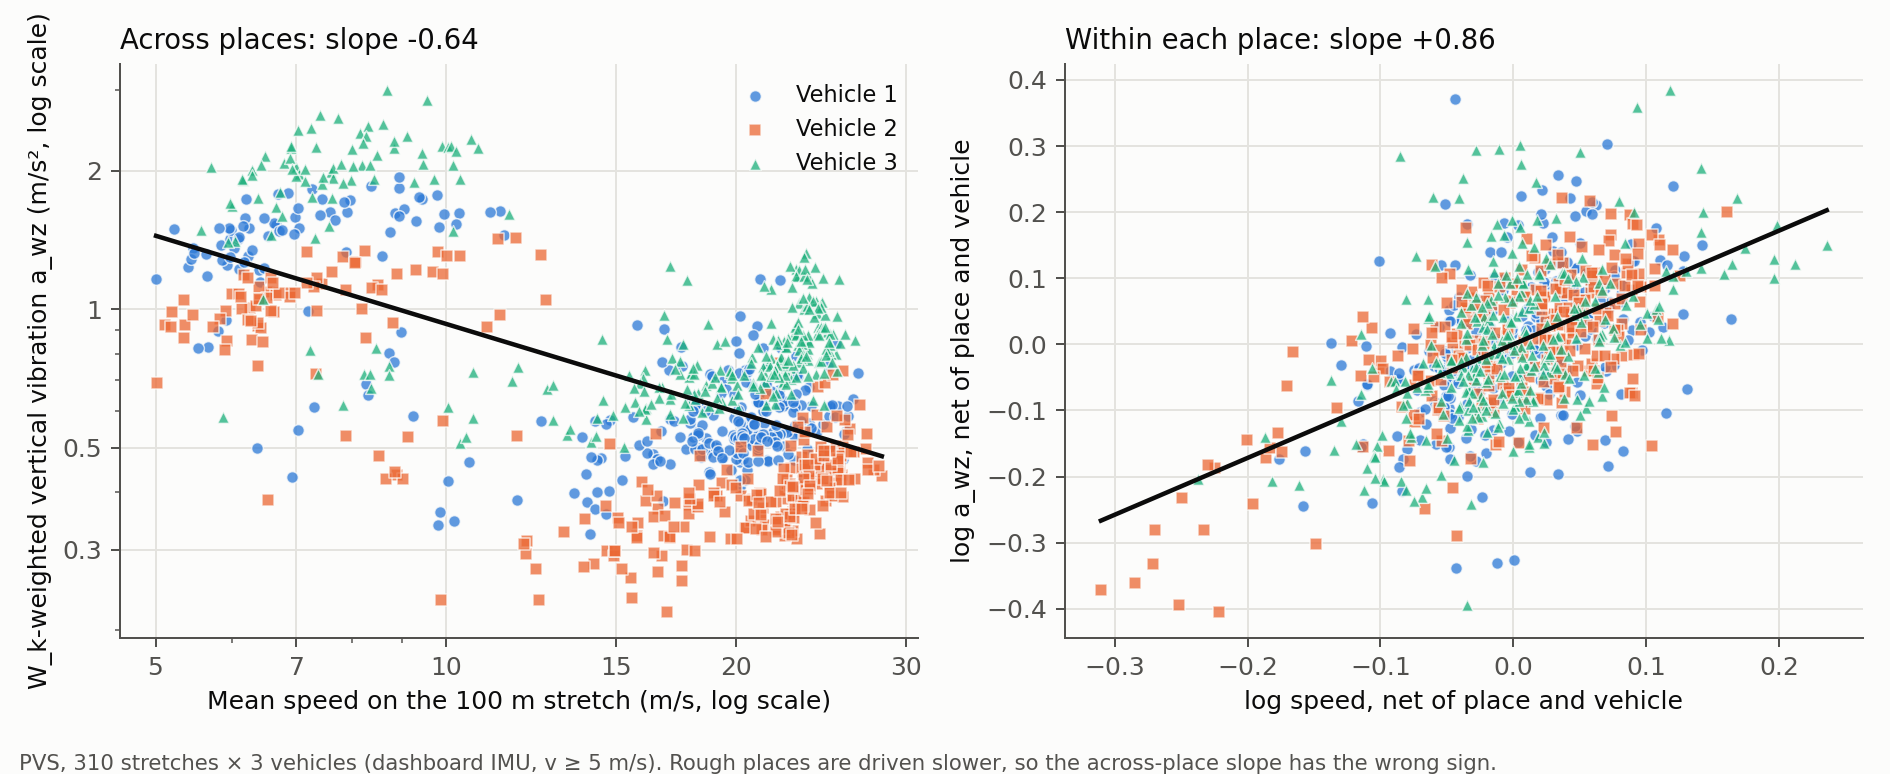
\includegraphics[width=\linewidth]{fig_speed.png}
\caption{Speed elasticity of dashboard vibration at 310 places, three vehicles. Left: across places (pooled OLS, slope $-0.64$). Right: within places, net of place and vehicle (partial-regression plot of Eq.~\eqref{eq:fe}, slope $+0.86$).}
\label{fig:speed}
\end{figure}

\subsection{Calibration on shared roads}
\label{sec:calibration}
\TBD[: P4 results: leave-one-route-out calibration of $\hat g_c$ and $\hat\gamma$; agreement of calibrated road classes; template narratives before/after (contradictions per co-located stretch pair and number of claims); P2 gain-only vs spectral; P3 forward prediction.]
